\section{Matrix-free GPU kernels}
In this chapterr, we develop custom, matrix-free GPU kernels (specifically for SBP-SAT methods) for computations in the volume and boundaries, which show improved performance as compared to the native, matrix-explicit implementation while requiring only a fraction of memory. GPU-acceleration of our resulting matrix-free, preconditioned iterative scheme shows superior performance compared to state-of-the-art methods offered by NVIDIA.

Stencil computations have proven efficient in utilizing GPU resources to achieve optimal performance \citep{vizitiu2014optimized,krotkiewski2013efficient}. In this work we implement a similar GPU kernel for our 2D problem by matching each spatial node to a GPU thread, however, our work requires specialized treatment for domain boundaries. The most computationally expensive operator is the volume operator $\tilde{\boldsymbol{M}}^{c_{ij}}_{ij}$, which differs from traditional finite difference operators in that it involves derivative approximations at domain boundaries. However, the use of else statements in GPU kernels tends to lead to warp divergence and should be avoided. We construct the matrix-free action of $\boldsymbol{A}$, referred to as {\ttfamily mfA!}() based on node location. Kernel \autoref{alg:mfA-1} provides the partial pseudocode, i.e. it includes pseudocode for the $\tilde{\boldsymbol{M}}^{c_{ij}}_{ij}$ calculation; boundary condition calculations are further detailed in code block 1.  At interior nodes the action of $\tilde{\boldsymbol{M}}^{c_{ij}}_{ij}$ is defined by a single stencil (with spatially varying coefficients). The action of $\tilde{\boldsymbol{M}}^{c_{ij}}_{ij}$ on boundary nodes, however, has a different stencil depending on the face number and whether the node is at a corner of the domain. To avoid race conditions at corners (while minimizing conditional statements), only normal components of $\tilde{\boldsymbol{M}}^{c_{ij}}_{ij}$ are computed (as they correspond to the same stencil). For example on face 1 only the action of $\tilde{\boldsymbol{M}}^{c_{rr}}_{rr}$ and $\tilde{\boldsymbol{M}}^{c_{rs}}_{rs}$ are computed at the corners, see \autoref{fig:dots}. The action of the remaining components of $\tilde{\boldsymbol{M}}^{c_{ij}}_{ij}$ on the corner nodes are computed in computations associated with adjacent faces (faces 3 and 4). 

\begin{figure}
    \centering
    % \includegraphics[width=\linewidth]{speed_comparison_chart_v2.pdf}
    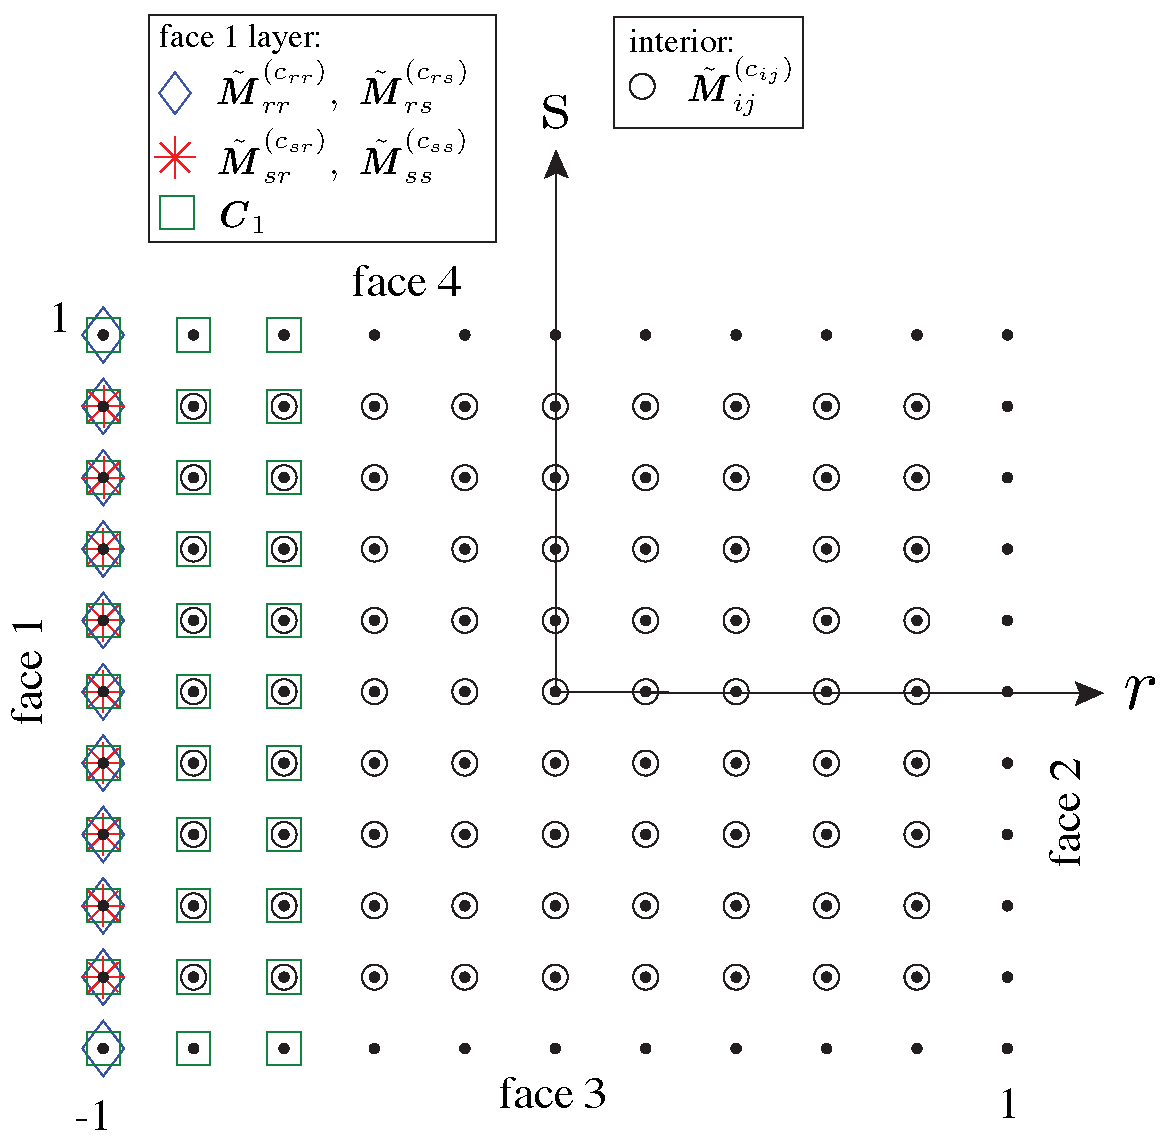
\includegraphics[width=\linewidth]{figures/dots_mod3.pdf}
    \caption{Schematic of 2D computational domain; nodes denoted with solid black dots. {\ttfamily mfA!}() modifies interior nodes, denoted with circles. For face 1, contributions to {\ttfamily mfA!}() from coordinate transformation matrices modify nodes corresponding to different shapes. Calculations by boundary operator $\boldsymbol{C}_1$ modify nodes in green squares.}
    \label{fig:dots}
\end{figure}


At boundary nodes we must also compute boundary condition operators $\boldsymbol{C}_k$, with differing stencils depending on face number and whether a node is an interior node, an interior boundary node (i.e. not a corner), or a corner node. Code block 1 provides the pseudocode for nodes on face 1; stencils are differentiated with superscripts $int, sw, nw$, corresponding to the interior boundary, northwest, and southwest corner nodes, respectively. \autoref{fig:dots} further illustrates the nodes involved in each computation: black dots correspond to nodes within the 2D domain. Black circles correspond to the interior nodes that are modified by the action of $\tilde{\boldsymbol{M}}^{c_{ij}}_{ij}$. On the western boundary (face 1), the three-node layer adjacent to face 1 is used to compute the actions of the volume and boundary operators.  Blue diamonds and red stars correspond to nodes that are modified by the different components of $\tilde{\boldsymbol{M}}^{c_{ij}}_{ij}$. Green squares correspond to the nodes that are modified by the boundary operator $\boldsymbol{C}_1$ in order to impose the Dirichlet condition (in this case a layer of three nodes normal to the face. More rows are involved for higher order $p$). 

% \setcounter{algorithm}{1}
\begin{algorithm*}
\caption{Matrix-Free GPU kernel Action of matrix-free A for interior nodes.}\label{alg:mfA-1}
\algrenewcommand\algorithmicprocedure{\textbf{function}}
\begin{algorithmic}
\Procedure{\textnormal{mfA!}}{\textnormal{odata}, \textnormal{idata}, $c_{rr}, c_{rs}, c_{ss}, h_r, h_s$}
    \State  $i, j = $get\_global\_thread\_IDs()
    \State $g = (i-1) * (N+1) + j$\Comment{compute global index}
    \If{$2 \leq i, j \leq N$} \Comment{\textnormal{interior nodes}}
        \State odata[g] = (\emph{hs}/\emph{hr})(- (0.5$c_{rr}$[$g$-1] + 0.5$c_{rr}$[$g$])\text{idata}[$g$-1] +
        \State \hspace{25mm}    + (0.5$c_{rr}$[$g$-1]  +  $c_{rr}$[$g$] - 0.5$c_{rr}$[$g$+1])\text{idata}[$g$] + 
        \State  \hspace{25mm}     - (0.5$c_{rr}$[$g$] + 0.5$c_{rr}$[$g$+1])\text{idata}[$g$+1]) + \\ \Comment{compute $M_{rr}$  stencil}\\
        \State \hspace{25mm} + 0.5$c_{rs}$[$g$-1](-0.5\text{idata}[$g$-$N$-2] + 0.5\text{idata}[$g$+$N$]) + 
        \State   \hspace{25mm} - 0.5$c_{rs}$[$g$+1](-0.5\text{idata}[$g$-$N$] + 0.5\text{idata}[$g$+$N$+1]) + \\ \Comment{compute $M_{rs}$  stencil}\\
        \State  \hspace{25mm} + 0.5$c_{rs}$[$g$-$N$-1](-0.5\text{idata}[$g$-$N$-2] + 0.5\text{idata}[$g$-$N$]) + 
        \State  \hspace{25mm} - 0.5$c_{rs}$[$g$+$N$+1](-0.5\text{idata}[$g$-$N$] + 0.5\text{idata}[$g$+$N$+2]) + \\ \Comment{compute $M_{sr}$  stencil}\\
        \State  \hspace{25mm} - (0.5$c_{ss}$[$g$-$N$-1] + 0.5$c_{ss}$[$g$])\text{idata}[$g$-$N$-1] + 
        \State  \hspace{25mm} + (0.5$c_{ss}$[$g$-$N$-1]  + $c_{ss}$[$g$] + 0.5$c_{ss}$[$g$+$N$+1])\text{idata}[$g$] - 
        \State  \hspace{25mm}     - (0.5$c_{ss}$[$g$] + 0.5$c_{ss}$[$g$+$N$+1])\text{idata}[$g$+$N$+1])) \\
        \Comment{compute $M_{ss}$  stencil}
    \EndIf
    \State  \dots \Comment{boundary nodes, e.g. Algorithm \autoref{alg:mfA-2}}
    \State \textbf{return} $nothing $ 
\EndProcedure
\end{algorithmic}
\end{algorithm*}


% \setcounter{algorithm}{2}
\begin{algorithm*}
\caption{Matrix-Free GPU kernel Action of matrix-free A for west boundary (face 1).}
\label{alg:mfA-2}
\begin{algorithmic}
\If{$2 \leq i \leq N$ \textnormal{and} $j = 1$} \Comment{\textnormal{interior west nodes}}
\State odata[$g$] = $\left(M_{rr}^{int} + M_{rs}^{int} + M_{sr}^{int} + M_{sr}^{int} + C_1^{int}\right)(\textnormal{idata})$ \\ \Comment{apply boundary $M$ and $C$ stencils}
\State  odata[$g$+1] = $C_1^{int}(\textnormal{idata})$\Comment{apply interior $C$ stencil}
\State odata[$g$+2] = $C_1^{int}(\textnormal{idata})$\Comment{apply interior $C$ stencil}
\EndIf
\If{$i = 1$ \textnormal{and} $j = 1$} \Comment{\textnormal{southwest corner node}}
\State odata[$g$] = $\left(M_{rr}^{sw} + M_{rs}^{sw} + C_1^{sw}\right)(\textnormal{idata})$ \\ \Comment{apply southwest partial $M$ and $C$  stencils}
\State  odata[$g$+1] = $C_1^{sw}(\textnormal{idata})$\Comment{apply southwest interior boundary $C$  stencil}
\State odata[$g$+2] = $C_1^{sw}(\textnormal{idata})$\Comment{apply southwest interior boundary $C$  stencil}
\EndIf
\If{$i = N+1$ \textnormal{and} $j = 1$}\Comment{\textnormal{northwest corner node}}
\State odata[$g$] = $\left(M_{rr}^{nw} + M_{rs}^{nw} + C^{nw}\right)(\textnormal{idata})$ \\ \Comment{apply northwest partial $M$ and $C$ stencils}
\State odata[$g$+1] = $C^{nw}(\textnormal{idata})$\Comment{apply northwest interior boundary $C$  stencil}
\State odata[$g$+2] = $C^{nw}(\textnormal{idata})$\Comment{apply northwest interior boundary $C$  stencil}
\EndIf
\end{algorithmic}
\end{algorithm*}



\section{Performance: Matrix-free GPU kernels}
\subsection{Performance Comparison}\label{sec: comparison}
With {\ttfamily mfA!}() we can carry out the matrix-vector product without explicitly storing the matrix. In this section, we compare its performance against the matrix-explicit cuSPARSE SpMV implementation available through CUDA.jl. We note that this is not an exhaustive comparison against all possible sparse matrix data structures.  Our goal is to establish a baseline comparison of our matrix-free implementation against the standard sparse matrix format CSR in CUDA.jl, with a focus on integration with preconditioning for improving CG performance.  





We set up our benchmark as follows: We discretize the domain $\bar{\Omega}$ in each
direction using $N+1$ grid points, varying $N$ from $2^4$ to $2^{13}$, so the
matrix $\boldsymbol{A}$ is of size $(N+1)^2 \times (N+1)^2$. \autoref{fig:A100} and \autoref{fig:V100} compare the performance of the
matrix-free implementation against the matrix-explicit SpMV provided with
cuSPARSE using the CSR format on both the A100 GPU and V100 GPU.
The performance is measured by profiling 10,000 SpMV calculations with NVIDIA Nsight Systems, and the time results shown in the figures represent the time to perform one SpMV calculation.
For problem sizes large enough for GPUs with $N$ greater than $2^{10}$, we see consistent speedup from \texttt{mfA!()} kernel with higher speedup achieved for larger problem sizes. 
On the A100 GPU, our speedup ranges from $3.0\times$ to $3.1\times$, .
On the V100 GPU, we see a similar trend, with our speedup ranging from $3.1\times$ to $3.6\times$.

The {\ttfamily mfA!}() kernel has a low arithmetic intensity of $0.28$ based on the computation of the interior points (which accounts for more than $99\%$ of the total computation and data access).
This puts the {\ttfamily mfA!}() kernel in the bandwidth-limited regime~\citep{ding2019instruction}.
If we plot this on the Roofline model, as shown in \autoref{fig:roofline} as the left red dot, we see that our kernel achieves performance that is \emph{higher} than what is possible for the given arithmetic intensity.
If we calculate the arithmetic intensity based on the assumption that the data is read from the DRAM only \emph{once} (i.e., the ideal case when the kernel only incurs compulsory cache misses), as shown in \autoref{fig:roofline} as the right red dot, we see a higher arithmetic intensity of $1.85$ and our achieved performance falls below the Roofline.
This suggests that a large portion of our data is coming from the fast memory (e.g., L1 or L2 caches), leading to performance that is better than what can be achieved if the data is only coming from the DRAM.
%That said, the {\ttfamily mfA!}() still outperforms the SpMV kernel by a large margin, showing the value of the matrix-free SBP operator. 

To confirm our hypothesis, we use NVIDIA Nsight Compute to profile our code for the problem size of N=$2^{13}$.
The profile shows that we achieved $72\%$ L1 cache hit rate and $57\%$ L2 cache hit rate, which indicates that the majority of our data is coming from the L1 and L2 caches (approximately $88\%$), and that our DRAM reads are due mostly to compulsory cache misses (i.e., when the input data is read for the first time).
This explains why our code performs better than the DRAM-bounded performance.
\autoref{fig:roofline-double-precision} shows the Roofline model generated by Nsight Compute, based on performance counter measurements of how much of the overall data is coming from different levels of the memory hierarchy.
\autoref{fig:roofline-double-precision} confirms that the majority of our data comes from the L1 cache, followed by L2 and DRAM.
It also suggests that we can further improve the performance of our $\texttt{mfA!}$() kernel by improving data reuse in the L1 cache, which will yield up to $3.8\times$ speedup.


In future work, we will target improved performance of {\ttfamily mfA!}(), for example through additional memory optimization techniques to improve L1 cache hit rate, especially with respect to its performance on newer architectures. In the present work, however, we focus on utilizing {\ttfamily mfA!}() to solve the linear system with preconditioning.



\begin{figure}
    \centering
    % \includegraphics[width=\linewidth]{speed_comparison_chart_v2.pdf}
    % \includegraphics[width=\linewidth]{chart_edit.pdf}
    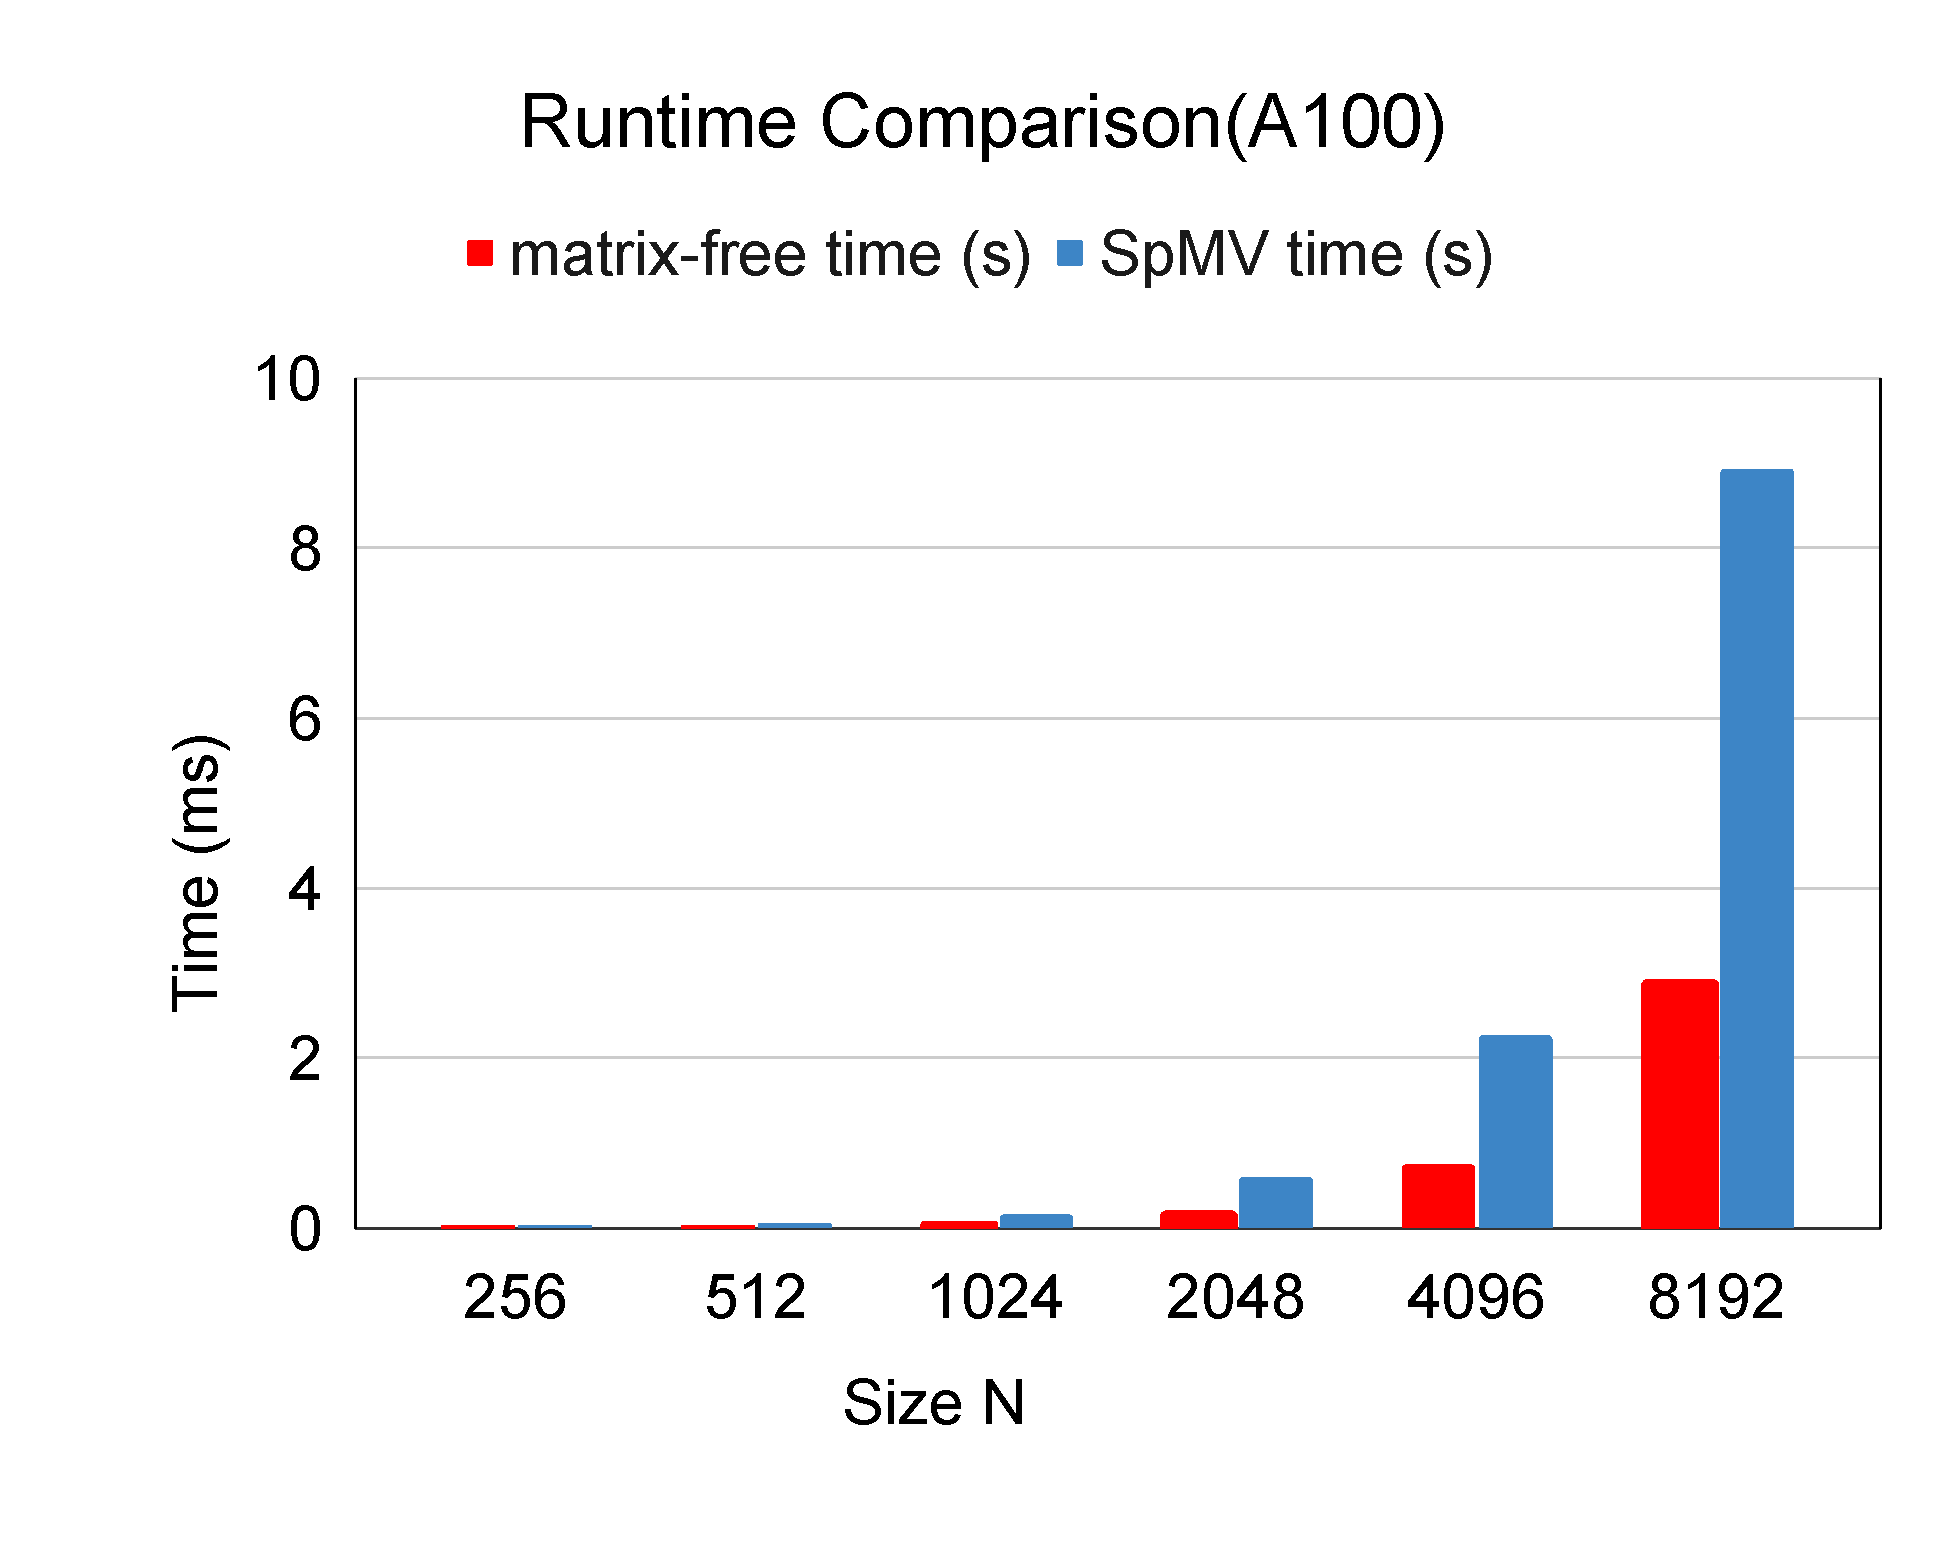
\includegraphics[width=\linewidth]{figures/Runtime_Comparison_A100.pdf}
    \caption{Performance of SpMV vs matrix-free $\texttt{mfA!}$() on A100 GPU. Total time for matrix-free (red) and matrix-explicit CSR (blue) formats are shown in charts plotted against $N$, where the matrix is size $(N+1)^2 \times (N+1)^2$.}
    \label{fig:A100}
\end{figure}

\begin{figure}
    \centering
    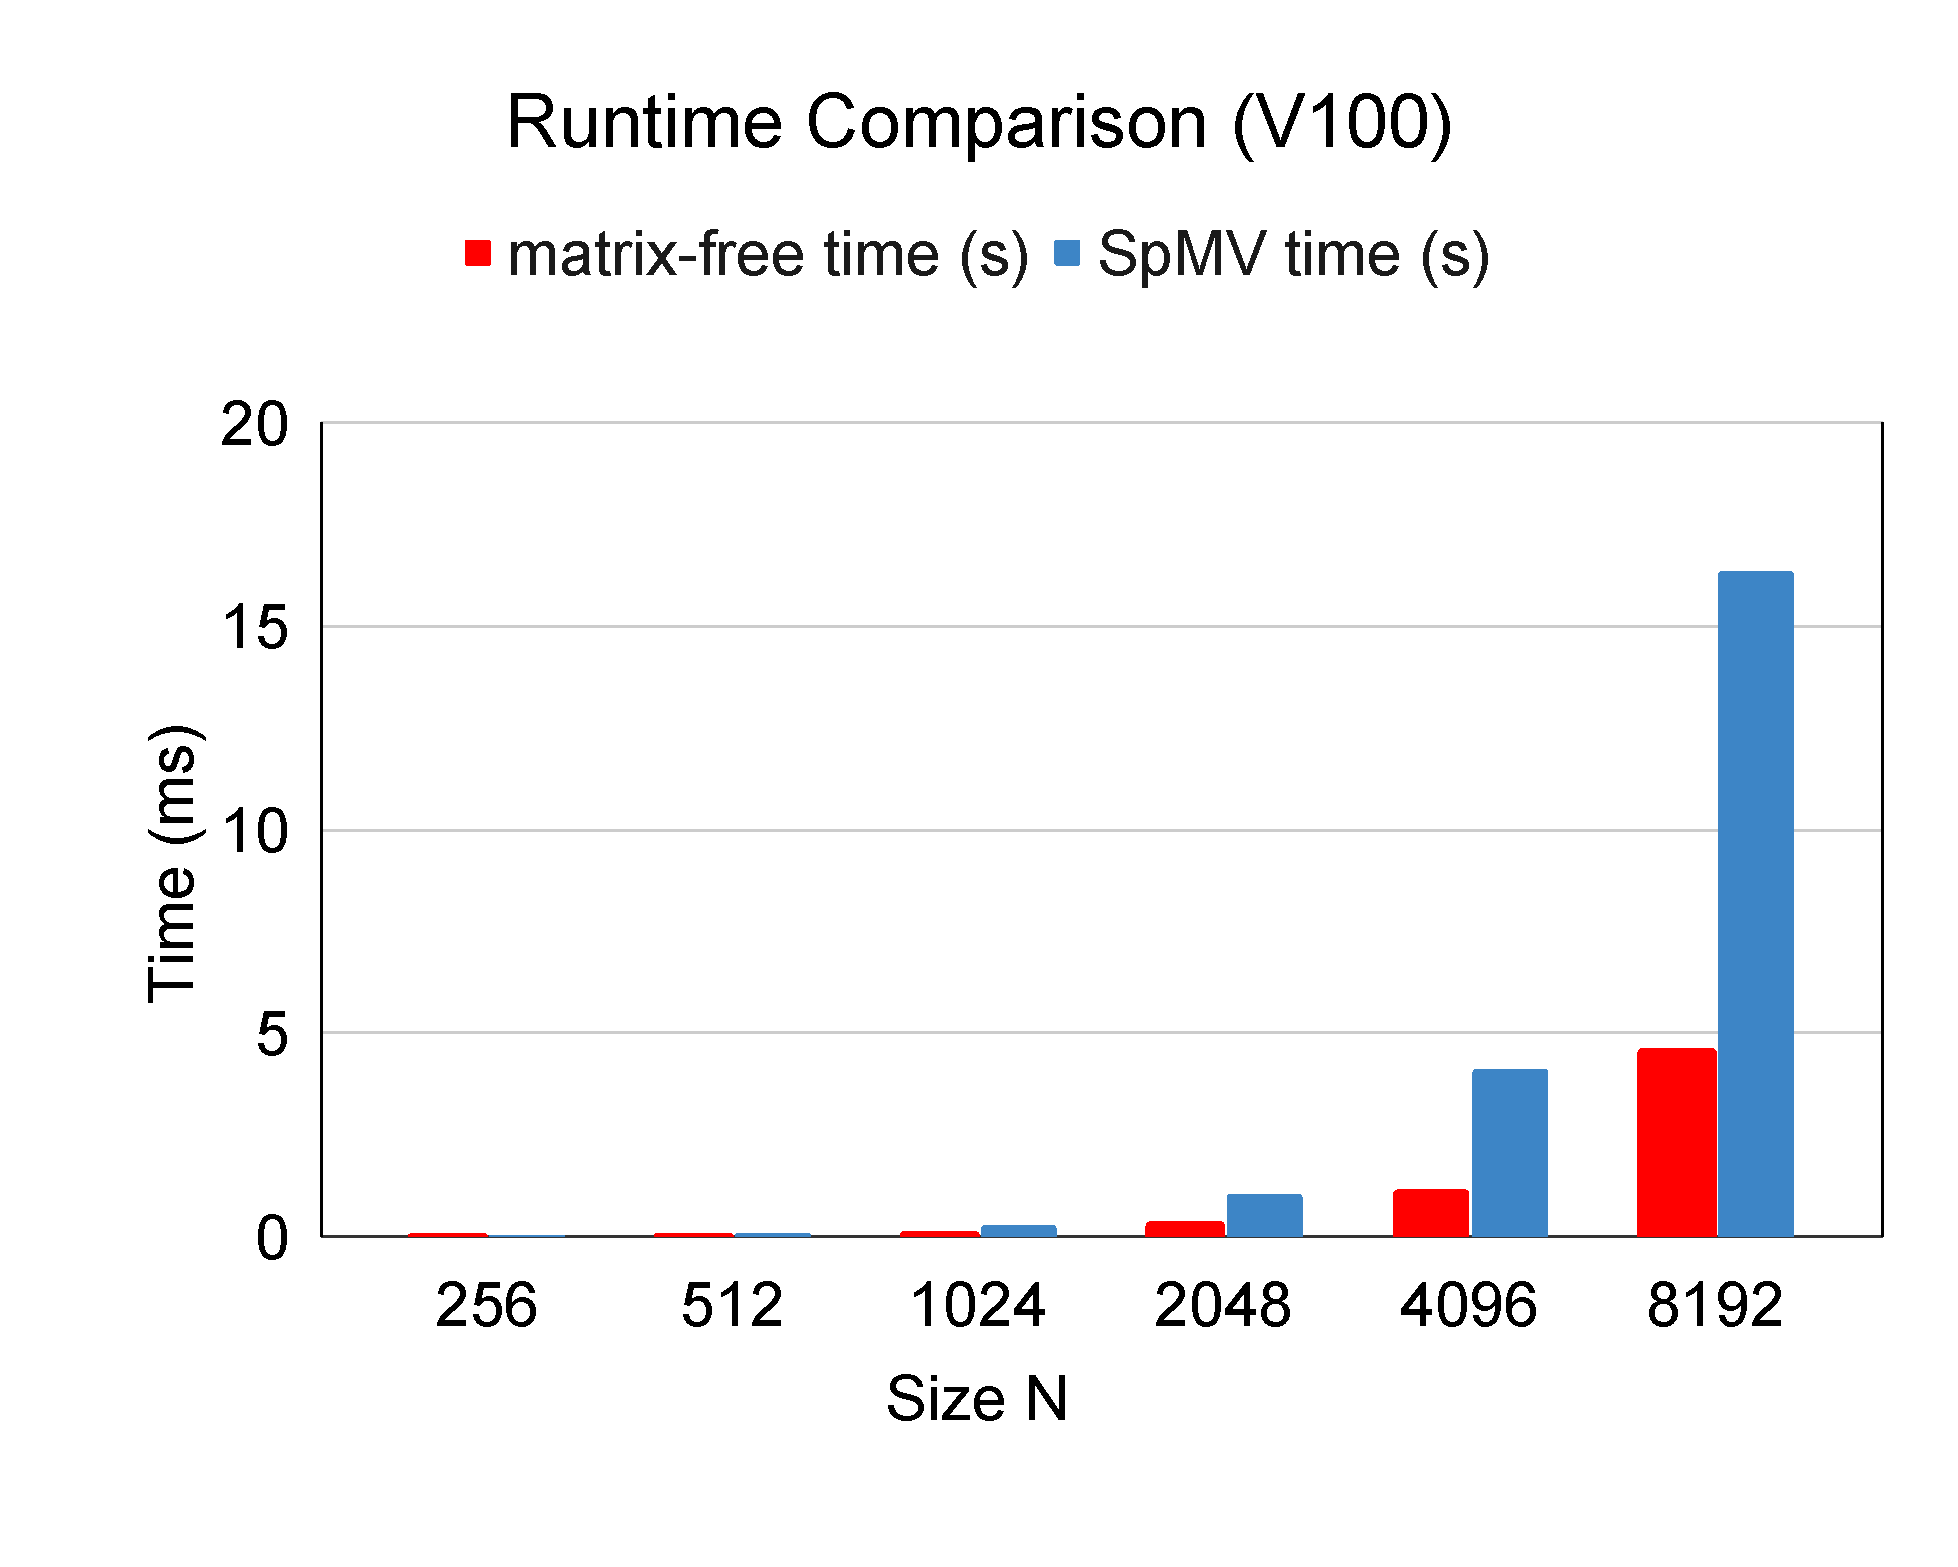
\includegraphics[width=\linewidth]{figures/Runtime_Comparison_V100.pdf}
    \caption{Performance of SpMV vs matrix-free $\texttt{mfA!}$() on V100 GPU. Total time for matrix-free (red) and matrix-explicit CSR (blue) formats are shown in charts plotted against $N$, where the matrix is size $(N+1)^2 \times (N+1)^2$.}
    \label{fig:V100}
\end{figure}

\begin{figure}
    \centering
    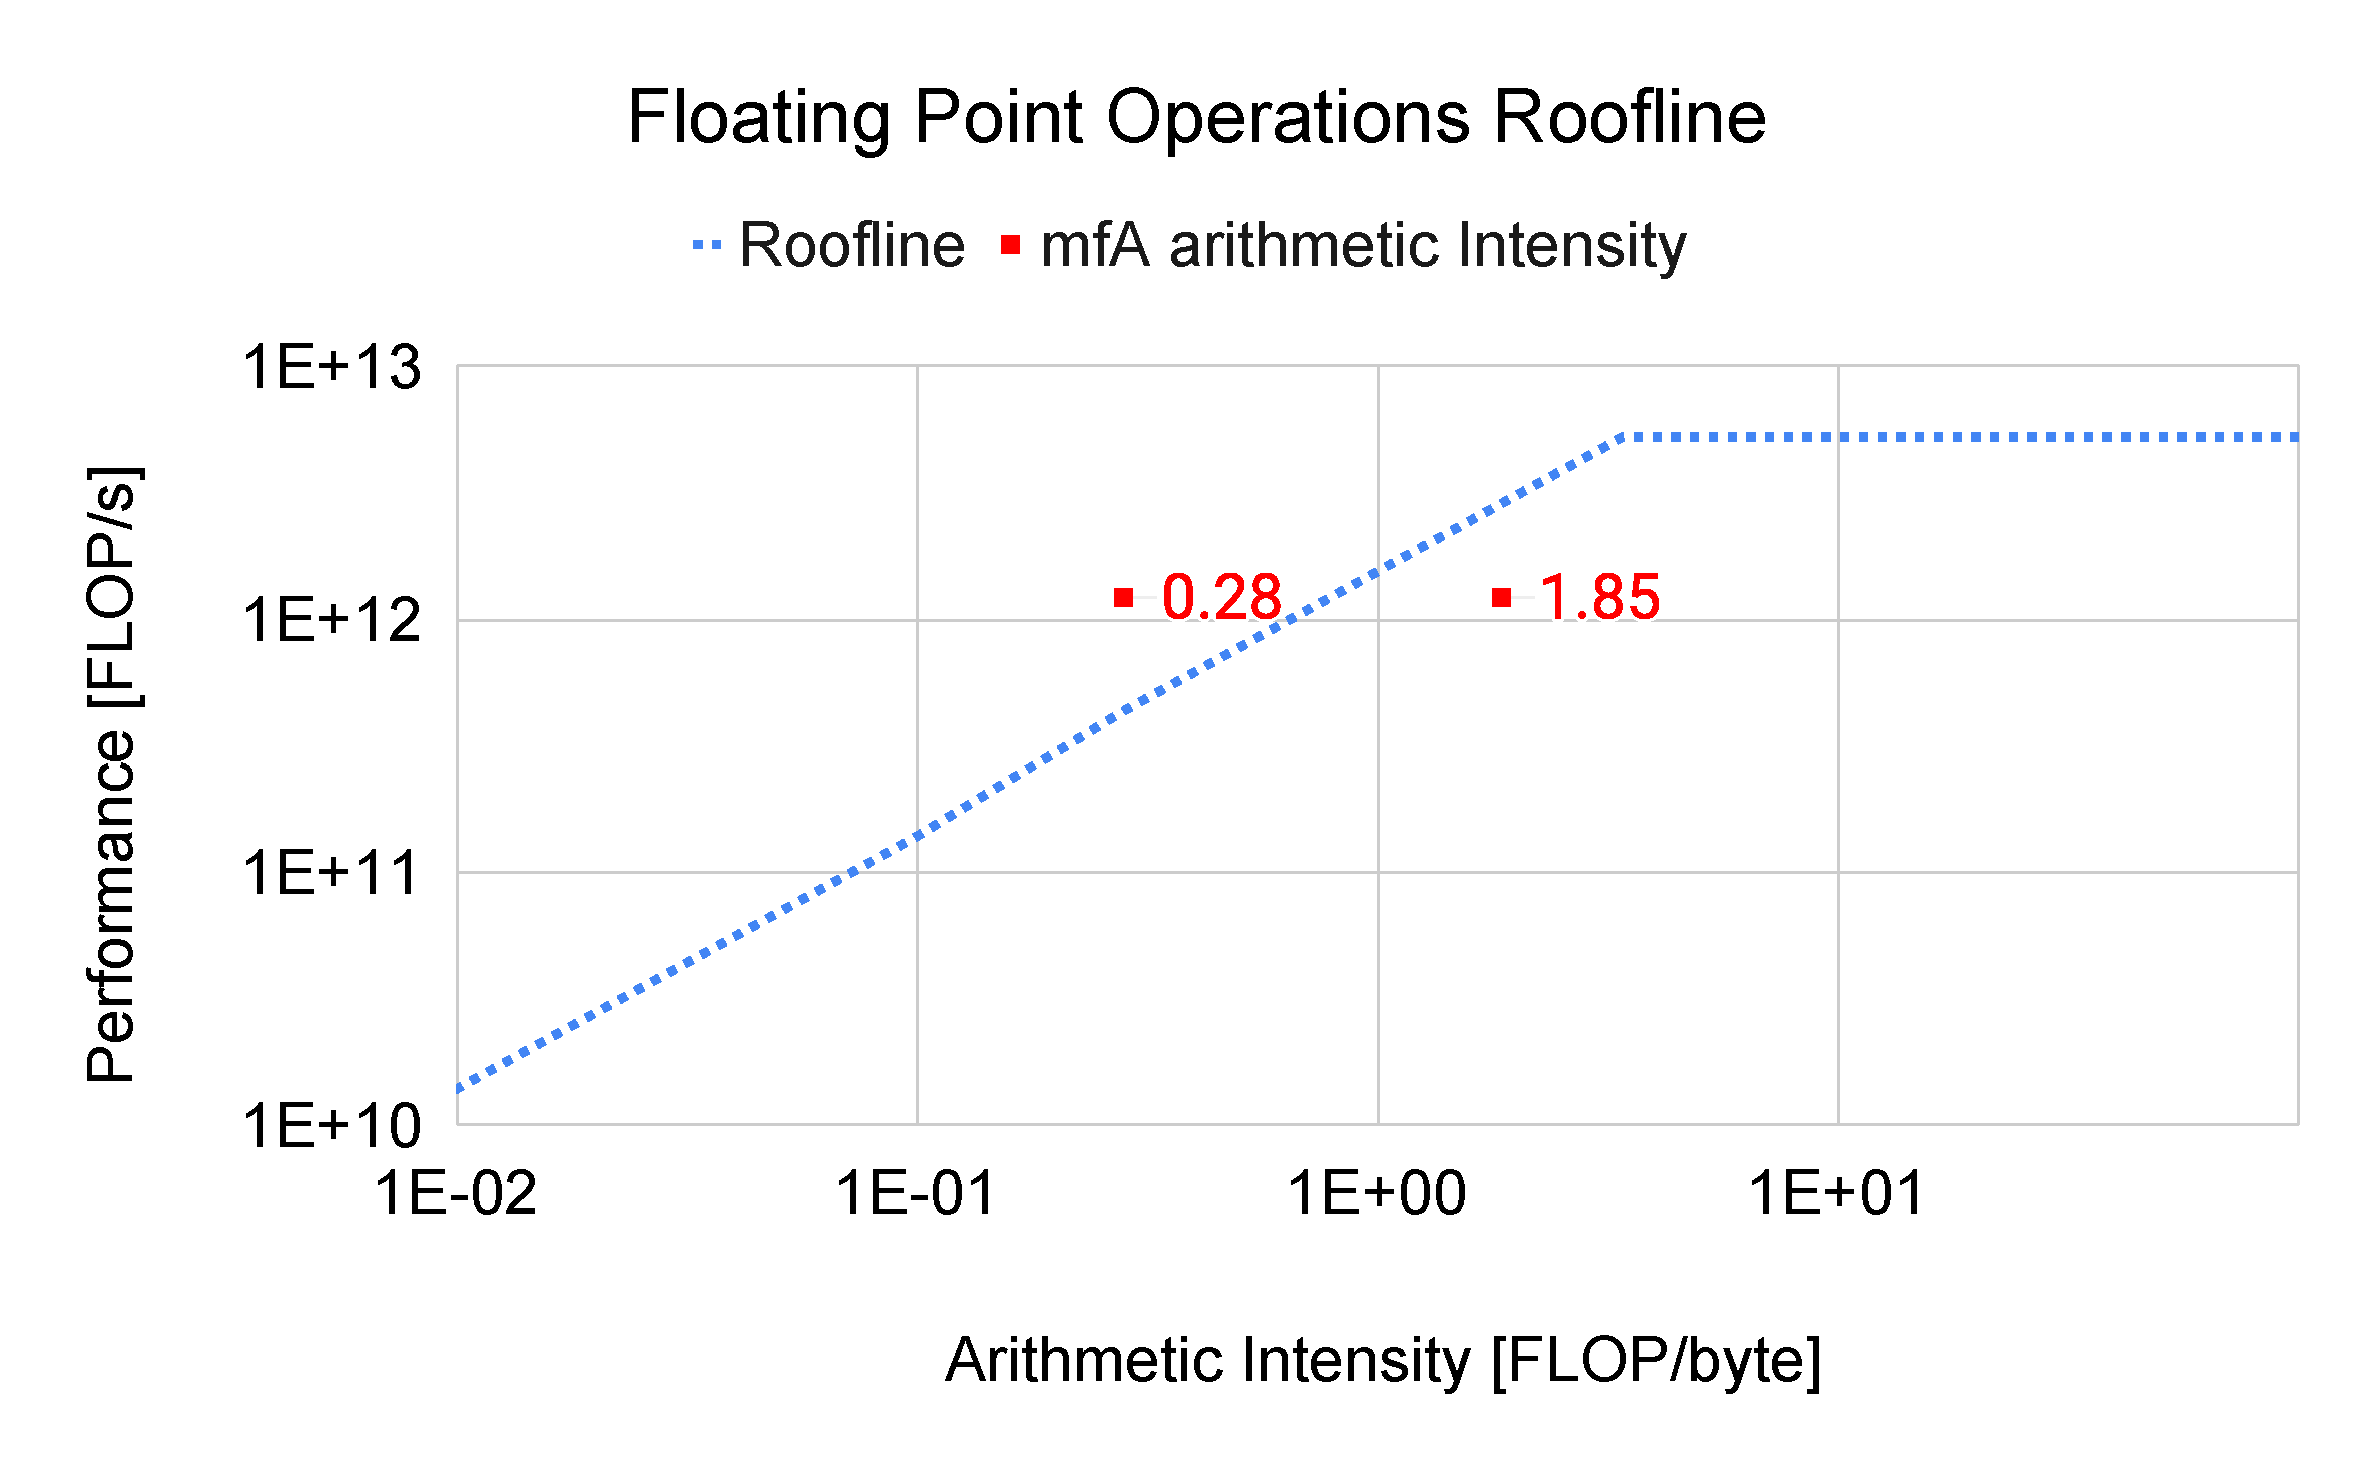
\includegraphics[width=\linewidth]{figures/Floating_Point_Operations_Roofline_Theoretical.pdf}
    \caption{
    Roofline model analysis for our matrix-free $\texttt{mfA!}$() on the A100 GPU.
    The red dot on the left represents the performance achieved by our kernel and its arithmetic intensity (0.28).
    The red dot on the right represents the same but assuming data is loaded only once from DRAM (i.e., compulsory misses), which yields a higher arithmetic intensity (1.85).
    The fact that our kernel (red dot) achieves higher performance than what is predicted by the Roofline model suggests that a large portion of our data is coming from the caches.
    %Roofline analysis for double-precision achieved value from Nsight Compute (blue dotted line) for the matrix-free kernel and theoretical arithmetic intensity for mfA kernels (red points). The left point counts all memory accesses to L1, L2 caches, and DRAM. The right point counts only access to DRAM and assumes the mfA!() kernel reads each data from DRAM only once.
    }
    \label{fig:roofline}
\end{figure}

\begin{figure}
    \centering
    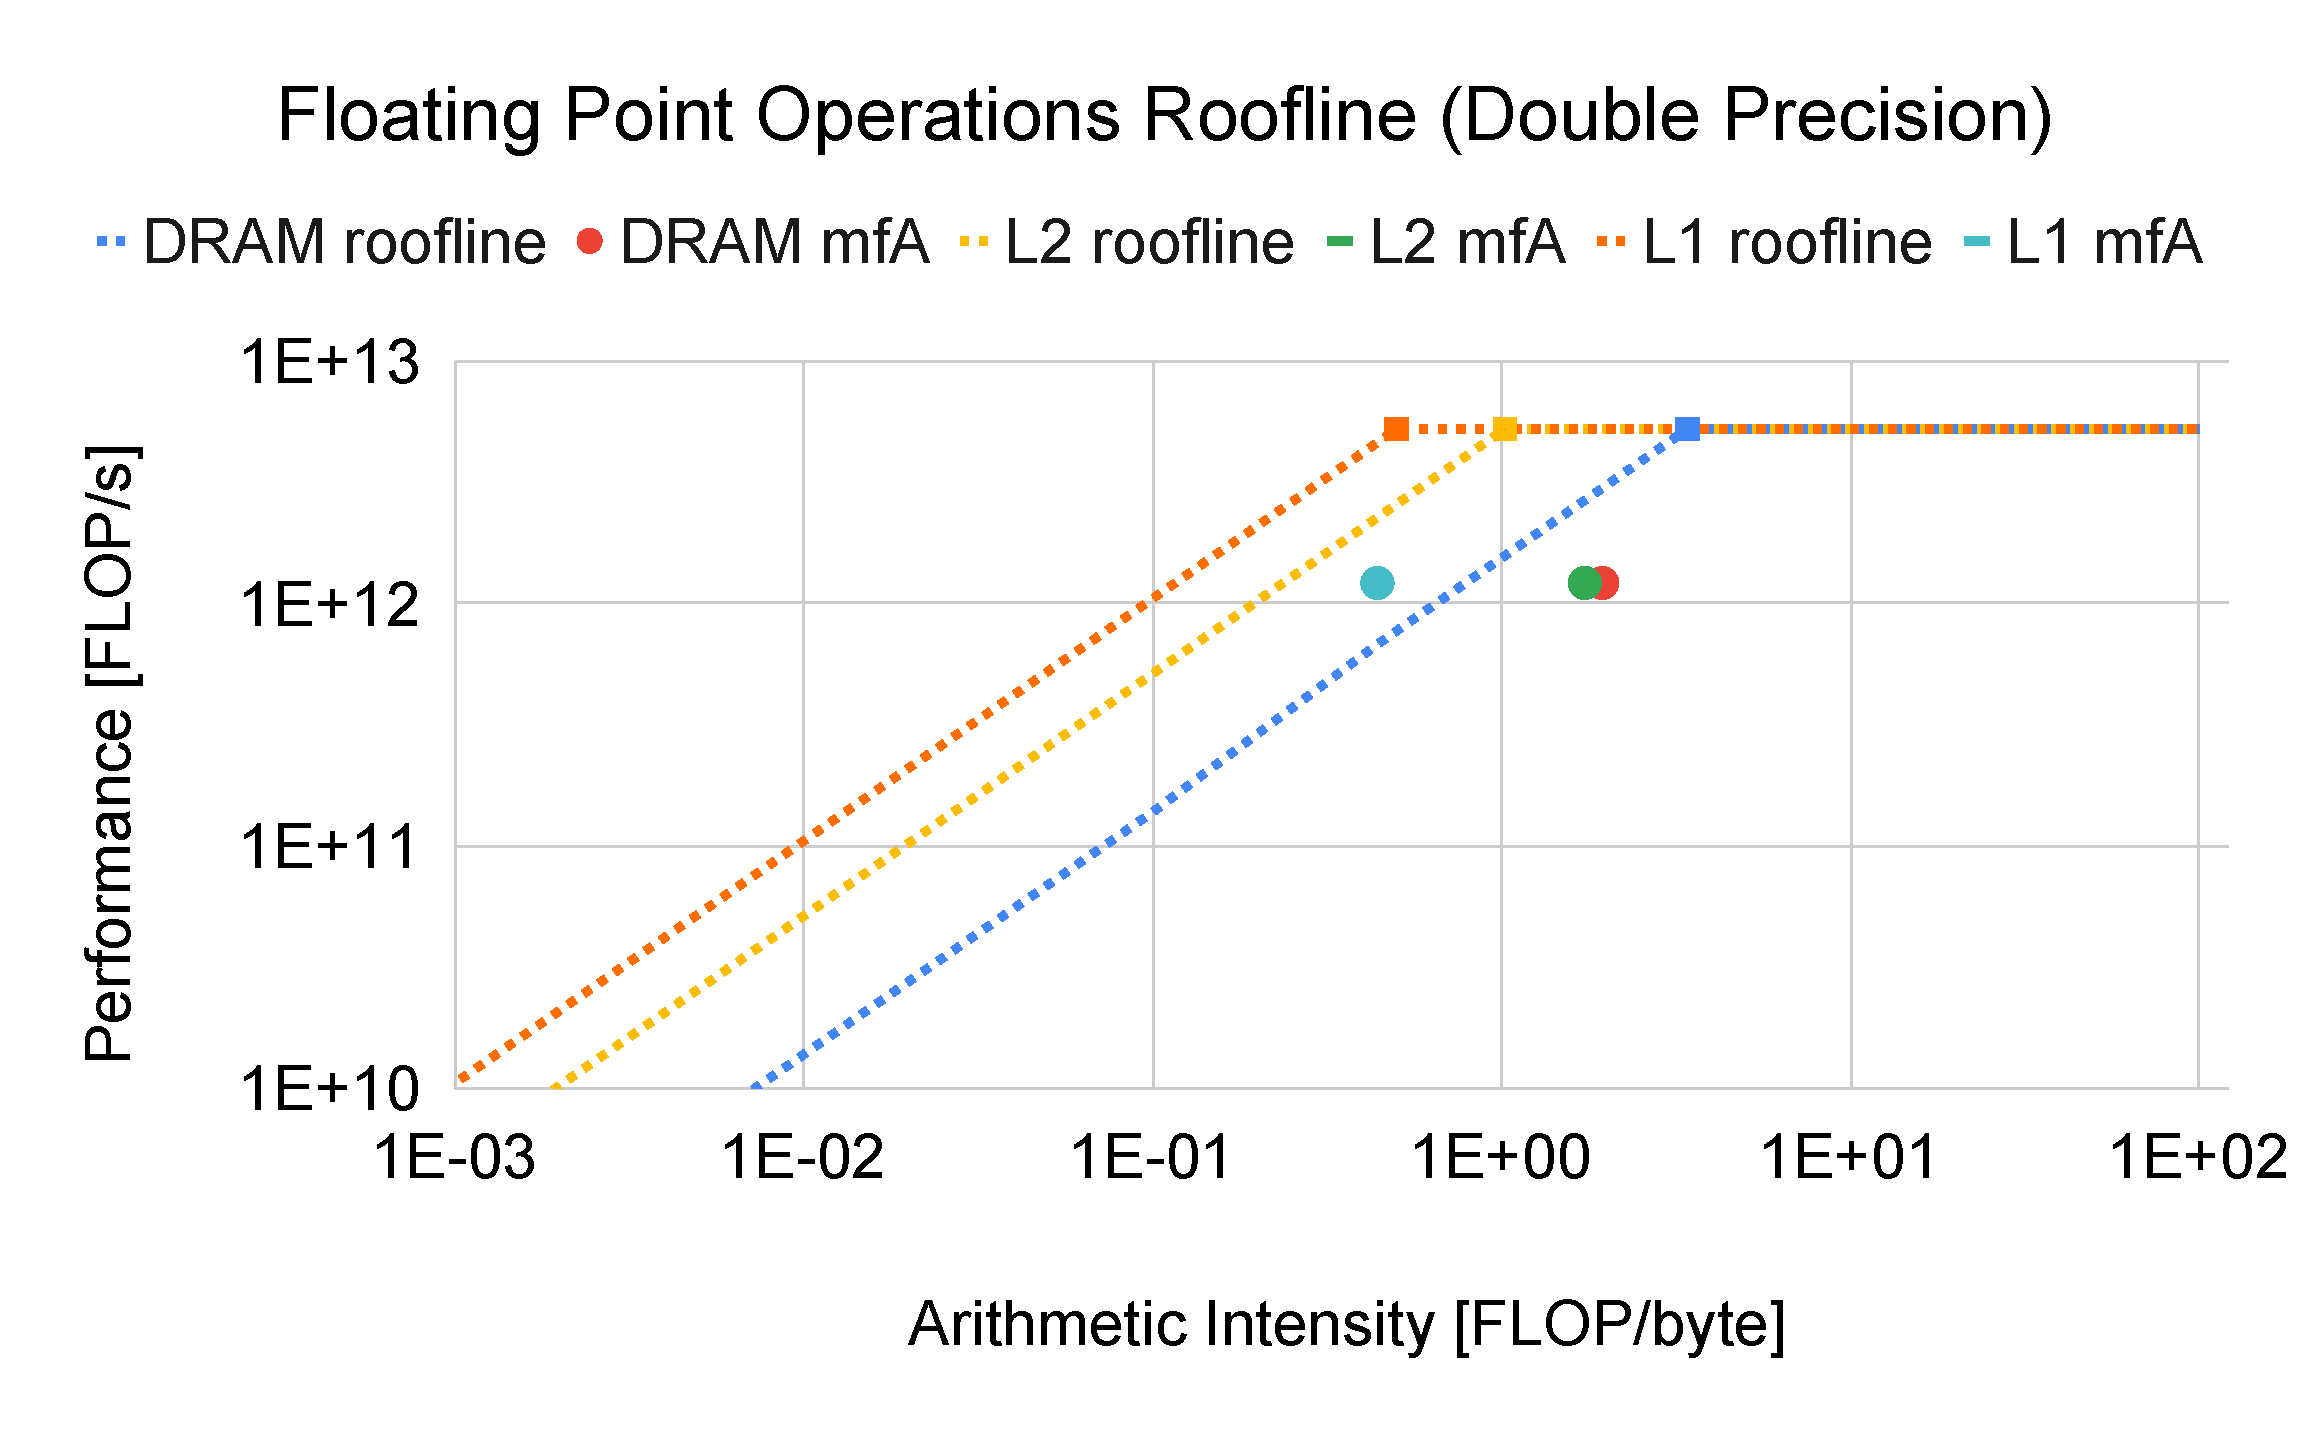
\includegraphics[width=\linewidth]{figures/Floating_Point_Operations_Roofline_Double_Precision.pdf}
    \caption{
    Roofline model generated by Nsight Compute, based on performance counter measurements of how much of the overall data is coming from different levels of the memory hierarchy.
    This confirms our hypothesis that the majority of our data is coming from the L1 cache, and that further improving data reuse in L1 will yield up to $3.8\times$ speedup.
    %Hierarchy roofline analysis for L1, L2, and DRAM (circles from left to right) double-precision achieved values from Nsight Compute for the matrix-free kernel.
    }
    \label{fig:roofline-double-precision}
\end{figure}




\subsection{Memory Usage Comparison}
Next we compare the memory usage of {\ttfamily mfA!}() against the SpMV kernel via the built-in memory status function in CUDA.jl. 
CUDA.jl currently has good support for only three different sparse matrices: CSR, CSC, and COO.
In Julia, the default sparse matrix format is CSC, but in CUDA.jl, the default sparse matrix format is CSR, and thus, there is a necessary conversion between these two formats when converting the CPU arrays to GPU arrays in Julia. 
%However, the actual memory requirement is very similar as these two formats are the transpose of each other. 
However, for our problem, where the matrix is SPD, both CSR and CSC formats use exactly the same amount of memory; the only difference is in the use of row pointer \texttt{rowptr} values (for CSR) instead of column pointer values \texttt{colptr} (for CSC), and the order of nonzero values \texttt{nzval}. 
%stored.
To avoid redundancy, we merge key results in memory consumption for CSC and CSR formats into three different numbers for each $N$.
The collected data is given in \autoref{tab:memalloc_comparison}. 
\label{sec:mem_comp}


\begin{table}[t]
\small\sf\centering
\begin{center}
\begin{tabular}{l l l l l }
\toprule
$N$  & m & nzval & memory size \\
\midrule
$2^{10}$& 1050625  & 9447429 & 0.1596 GB \\
$2^{11}$ & 4198401 & 37769221& 0.6379 GB &  \\
$2^{12}$ & 16785409   & 151035909   & 2.5509 GB &  \\
$2^{13}$ & 67125249   & 604061701   & 10.2020 GB & \\
\bottomrule
\end{tabular}
\end{center}
\caption{Number of nonzero values (nzval) for CSC or CSR sparse matrices with different $N$, where matrix size is $(N+1)^2 \times (N+1)^2$. The matrices are SPD. Here, m represents the number of rows, and nzval represents the number of nonzero values. The total memory size (last column) is calculated using previous columns.
}
\label{tab:memalloc_comparison}
\end{table}


\begin{table}[t!]
\small\sf\centering
\begin{center}
\begin{tabular}{l l l l l }
\toprule
$N$  & crr/css/crs & $\Psi_1$/$\Psi_2$ & total memory size \\
\midrule
$2^{10}$& 0.008405 GB  & 8 KB & 0.02523 GB \\
$2^{11}$ & 0.03359 GB & 16 KB &  0.1008 GB \\
$2^{12}$ & 0.1343 GB  & 32 KB  & 0.4029 GB &  \\
$2^{13}$ & 0.5370 GB   & 65 KB   & 1.6111 GB & \\
\bottomrule
\end{tabular}
\end{center}
\caption{Memory allocation for matrix-free methods where matrix size is $(N+1)^2 \times (N+1)^2$. Here $\mathrm{crr}$, $\mathrm{css}$, and $\mathrm{csr}$ correspond to coefficient matrices of size $(N+1)^2$. $\Psi_1$ and $\Psi_2$ are used in Dirichlet boundary conditions and are vectors of length $N+1$. Total memory allocated (last column) is calculated using previous columns.
}
\label{tab:memalloc_mf}
\end{table}

For the matrix-free method, memory consumption is reported in \autoref{tab:memalloc_mf}. 
In order to perform the matrix-vector product, we need to allocate memory to store the coefficients $c_{rr}$, $c_{ss}$ and $c_{rs}$; each requires the same size of memory as the numerical solution and must be stored on each grid level when using geometric multigrid as a preconditioner. 
In addition, we must compute and store the minimum coefficient values ${\boldsymbol{C}}_{rr}^{k, min}$ on faces 1 and 2, as specified in the previous section, which we denote $\Psi_1 = $ and $\Psi_2$, respectively. 


These are associated with Dirichlet boundary conditions and are significantly smaller in size, and thus reported in KB. Adding up these contributions, we can compute the total memory size, which we provide in the last columns of Tables \autoref{tab:memalloc_comparison} and \autoref{tab:memalloc_mf}: We can see that there is a significant reduction in additional required memory for the matrix-free method than the memory to store sparse matrices in CSC or CSR format. When calculating the total memory used for an SpMV operation (including writing results into output vectors), we need to add additional memory allocated for the input data and output data, which require the same memory as the coefficients (the first column of \autoref{tab:memalloc_mf}). A simple calculation can show that the total memory required when using an SpMV kernel is a constant $4.2\times$ of that required for the matrix-free method. 